\documentclass[10pt,a4paper]{article}
\usepackage[utf8]{inputenc}
\usepackage{amsmath}
\usepackage{amsfonts}
\usepackage{amssymb}
\usepackage{color}
\usepackage{graphicx}
\author{K.M.J. Jacobs (s4134621) \and Zhuoran Liu (s4594851) \and Ankur Ankan (s4753828)}
\title{Stochastic Optimal Control}

% Set all of these to false for the final document
\newif\ifrequirements
\requirementstrue
%\requirementsfalse

\usepackage{listings}

\begin{document}
\maketitle

\newpage
\tableofcontents
\newpage

\ifrequirements
\color{red}
\textbf{Document requirements shown by flag \texttt{requirementstrue}.}
\textbf{Set flag \texttt{requirementsfalse}.}

\color{blue}
\section{Guidelines for ML assignments}
Note: All reports should be handed in before the end of January 2017. Hard deadline is \textbf{January 31 at 23.59}. Any questions about the below points please contact me (Hans-Christian Ruiz). For the assignments please refer to the ML course page.

\subsection{Requirements to hand in the reports}
\begin{itemize}
\item Hand in each report as a SINGLE document with all figures, code, etc (other "extra" files will not be considered). Hand in printed in my post box (Ruiz, wing 8, ground floor).
\item In addition, hand in the code that can be run stand-alone. Send us an email with a zip-file containing the codes for all assignments. The zip-file should be named with the last names of all group members. Each code in the zip-file should be named as AssignmentName where AssignmentName is: Ising, BM, MNIST, Lasso, Control
\item Your name on each report and the name of the corresponding code file in the zip-file that you sent us via email.
\item The report should be well structured and clear.
\item Figures need to have a caption explaining in detail what they show. 6. No more than 8 pages (excluding references and code) with 12 pts font.
\end{itemize}

\subsection{Minimal requirements of the content}
The report for each exercise addresses following points:
\begin{itemize}
\item Introduction: summarizes the underlying theory and algorithm(s). It should be a short description of the theoretical background and expla- nation of the method considered (no more than a page!).
\item Problem statement: Itemizes a number of research questions that you address
\item Results: Detailed description of the different numerical studies that you have performed with plots and specification of the parameter settings (a) Precise, clear description of what you have done, with the used formulas and the argumentation of why you have done it; e.g. what measure of convergence you used, are there alternatives? (b) Figures with a detailed explanation of what the relevant results are (c) An analysis of the results (for example: is the result as expected? why?/why not? what does the result mean? etc...)
\item General discussion/Conclusions: A summary of the main findings and conclusions (no more than half page!)
\item Appendix: If the exercise requires to write a code, add the code in the appendix. The code should have the following characteristics (a) Well documented, comments! (b) Suitable structure for readability, e.g. indentation, proper (mnemonic) variable naming. 6. Note: The code will not be evaluated based on whether it is optimized or not, only if it is clearly readable. But, IT MUST RUN STAND- ALONE!
\end{itemize}

\color{black}
\fi

\newpage
\section{Introduction}
The main topic of this assignment is Stochastic Optimal Control. For many problems, it is analytically feasible to compute the optimal control for a given stochastic system. For some problems however, it is only possible to approximate optimal control. The first part of the assignment focusses on a controlled random walk which is one of the easiest problems to look at. The second part of the assignment focusses on the well-known mountain car problem. In the second part of the assignment, MCMC sampling will be applied to approximately compute the optimal control.

\section{Problem statement}
\subsection{Controlled random walk}
In the controlled random walk problem, the rate of change of the state is defined as follows:

\begin{equation}
dx = u dt + d\xi
\label{eq:crw_dx}
\end{equation}

The state has initial position $x$ at $t = 0$. The noise variance is $\langle d \xi^2 \rangle = \nu dt$.

There are two targets at $t = T$ at locations $x = \pm 1$. The end-cost function $\phi$ is defined such that it has delta peaks at the targets:

\begin{equation}
\phi(x(T)) = \begin{cases}
0 & x(T) = \pm 1\\
\infty & \mbox{otherwise}
\end{cases}
\label{eq:crw_phi}
\end{equation}

The optimal control for this problem satisfies:

\begin{equation}
u^{*}(t, x) = \frac{\tanh(x / (\nu (T - t)) - x}{T - t}
\label{eq:crw_u}
\end{equation}

The following research questions are discussed for the controlled random walk problem in this report:
\begin{itemize}
\item How does the optimal control depend on parameters $\nu$ and $T$ numerically?
\item How does the delayed choice mechanism work?
\end{itemize}

\subsection{Mountain car problem}
The following research questions are discussed in this report for the mountain car problem as described in the assignment:
\begin{itemize}
\item What is the optimal control policy for this problem?
\end{itemize}

\section{Results}
\subsection{Controlled random walk}
\subsubsection{How does the optimal control depend on parameters $\nu$ and $T$ numerically?}
If $\nu \rightarrow \infty$, then $\tanh(\frac{x}{\nu (T - t)}) \rightarrow 0$ and then $u^{*}(t,x) \rightarrow 0$. If there is a large amount of noise, the the control goes to $0$ and if $t \rightarrow T$, then there will be a large amount of control.

\subsubsection{How does the delayed choice mechanism work?}

\begin{figure}
\centering
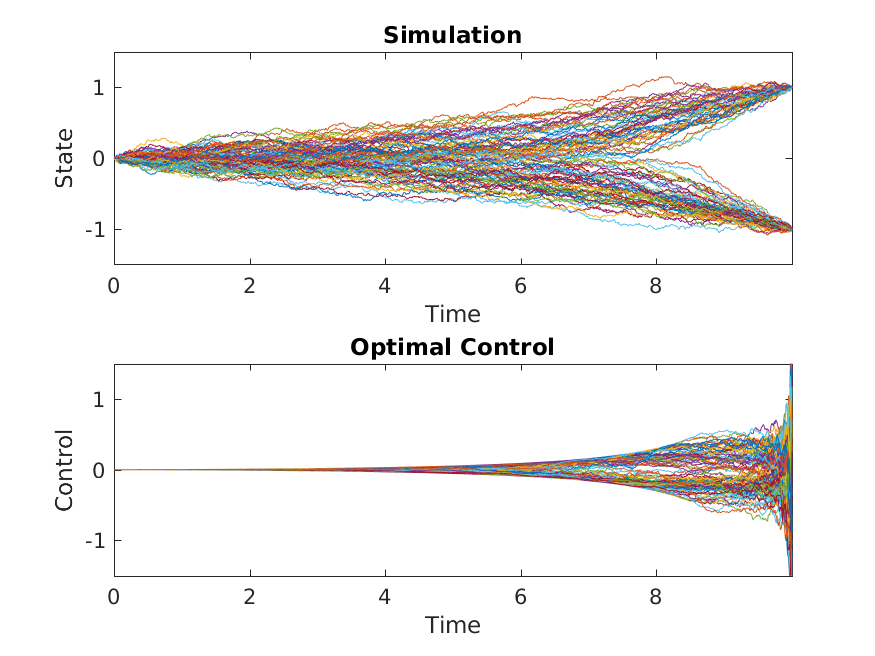
\includegraphics[width=300px]{crw-oc-1.png}
\caption{Optimal control for the Controlled Random Walk problem. With $\nu=0.1$, $T=10$, $dt=0.01$ for which $100$ trials are shown.}
\label{fig:crw-oc-1}
\end{figure}

There is no control unless it is clear that control can steer the system towards the optimal solution. It makes no sense to steer towards an optimum in a state in which the noise can push the state away from the optimal solution. Therefore, it is better to wait until it is ensured that control can steer the system to the optimal solution. This mechanism is shown in figure \ref{fig:crw-oc-1}.

\begin{figure}
\centering
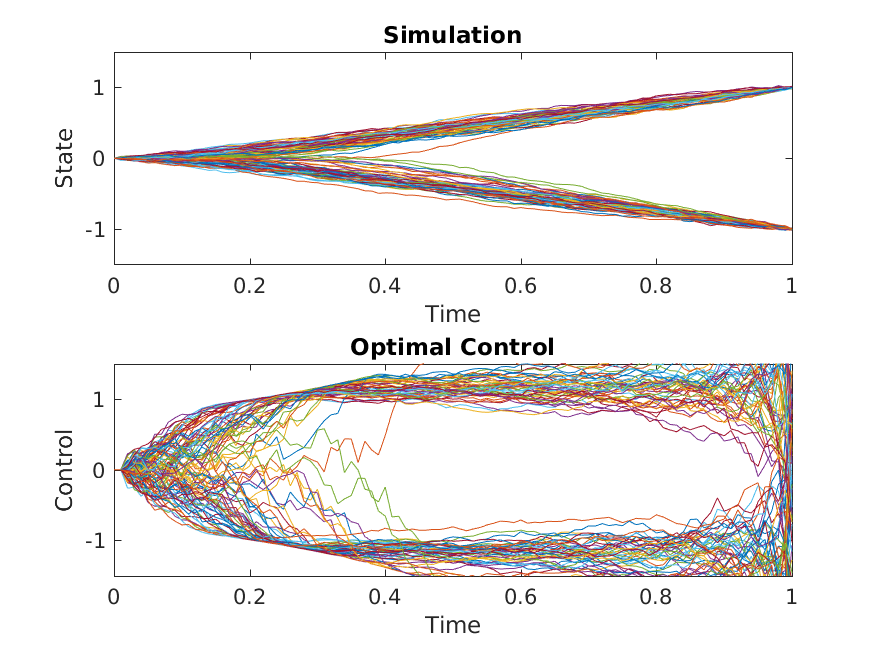
\includegraphics[width=300px]{crw-oc-2.png}
\caption{Optimal control for the Controlled Random Walk problem. With $\nu=0.1$, $T=1$, $dt=0.01$ for which $100$ trials are shown.}
\label{fig:crw-oc-2}
\end{figure}

If one would choose a lower horizon ($T = 1$ as in figure \ref{fig:crw-oc-2} instead of $T = 10$ as in figure \ref{fig:crw-oc-1}), the system has less time and thus less cumulative noise is expected. Therefore, it is advantageous to control the system at the start. Once the system has reached the optimal state ($x = -1$ or $x = 1$), it will steer the system such that it remains in the optimal state.

So when there is more time, there will be more cumulative noise and the system will delay its choice. If there is less time, it will be advantageous to steer the system towards to optimal state at the start.

\begin{figure}[h]
\centering
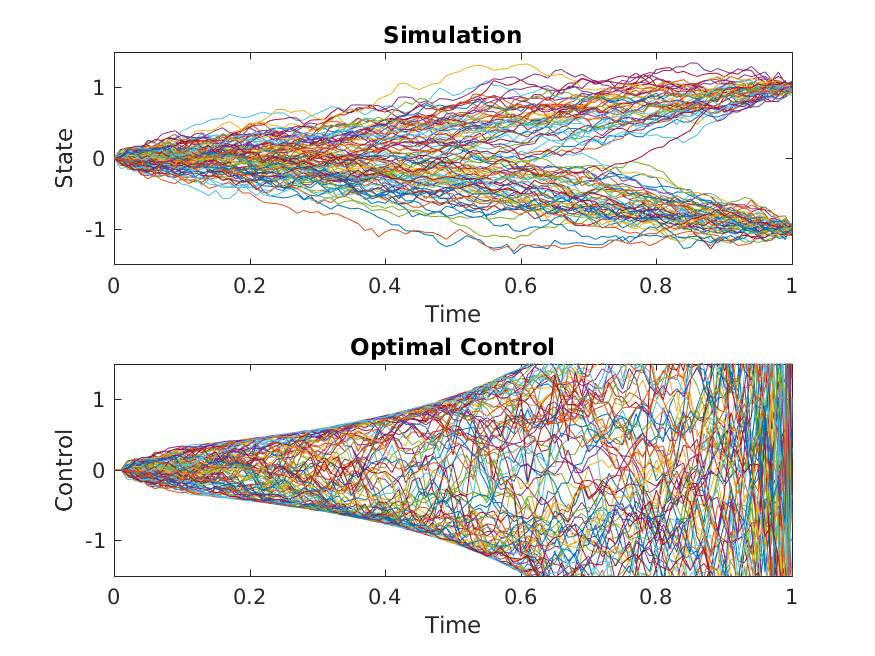
\includegraphics[width=300px]{crw-oc-3.png}
\caption{Optimal control for the Controlled Random Walk problem. With $\nu=0.5$, $T=1$, $dt=0.01$ for which $100$ trials are shown.}
\label{fig:crw-oc-3}
\end{figure}

If, however, there is more noise, the system will try to keep the system stable from the beginning on by steering the system such that the optimum remains in reach. So, up to some level, more noise results into larger control. This can be seen by comparing figure \ref{fig:crw-oc-2} to figure \ref{fig:crw-oc-3}.

\subsection{Mountain car problem}
For the first part of the mountain car problem assignment, it is asked to find parameters with $(x_0, v_0) = (0.5, 0)$ such that the problem is too easy and all trajectories reach the top of the hill and it is asked to find parameters such the problem is harder, but still some trajectories will reach the top of the hill.

First, it is easy to gain some insights by plotting the graph for the hill $L(x)$ and by visualizing the gravitational force $F_g(x)$.

\begin{figure}[h]
\centering
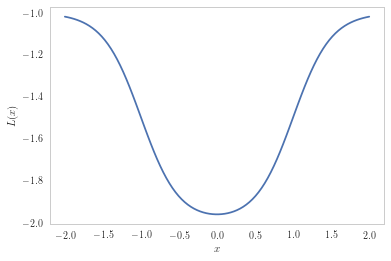
\includegraphics[width=150px]{lx.png}
\caption{The plot of the hill $L(x)$.}
\label{fig:mcp-fgx}
\end{figure}

\begin{figure}[h]
\centering
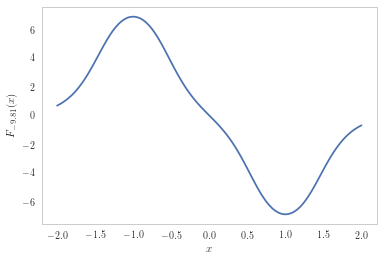
\includegraphics[width=150px]{fgx.png}
\caption{The gravitational force $F_g(x)$ for $g=-9.81$.}
\label{fig:mcp-fgx}
\end{figure}

What can be seen from the formula of $F_g(x)$, is that the derivative of $L(x)$ forces the car to either go back to the bottom of the valley (this happens when $g < 0$ or it pushes the car further up the hill (when $g > 0$). With $g = 0$, there is no gravitational force at all.

\begin{figure}[h]
\centering
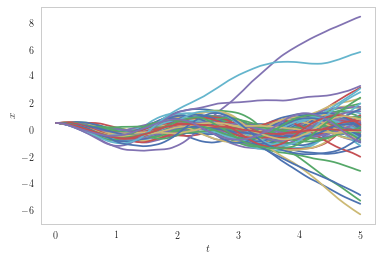
\includegraphics[width=150px]{sim_g10.png}
\caption{100 simulations for $x_0 = 0.5$, $v_0=0$, $\nu=1$, $T=5$ and $g=-10$.}
\label{fig:mcp-g10}
\end{figure}

\begin{figure}[h]
\centering
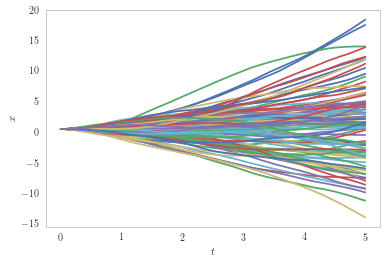
\includegraphics[width=150px]{sim_g0.png}
\caption{100 simulations for $x_0 = 0.5$, $v_0=0$, $\nu=1$, $T=5$ and $g=0$.}
\label{fig:mcp-g0}
\end{figure}

In figures \ref{fig:mcp-g10} and \ref{fig:mcp-g0}, it can be seen that $g \neq 0$ forces the car back to the bottom of the valley. $g=0$ has no influence on the trajectories and does not necessarily keep the trajectories in the valley. For large values of $\nu$, it is more often the case that trajectories escape the valley. If the noise is extremely large, then the car escapes the valley fairly quickly. By the large noise, it is unlikely that the car is accidentally pushed back into the valley.

\begin{figure}[h]
\centering
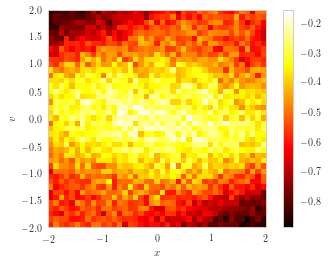
\includegraphics[width=150px]{J.png}
\caption{The optimal cost-to-go at $t=0$, $\nu=4$, $g=-10$ and without control (so $u=0$) computed by calculating $100$ simulations per $(x_0, v_0)$ pair.}
\label{fig:mcp-j}
\end{figure}

For the second part of the second part of the assignment, it is asked to compute the optimal cost-to-go $J(x, v, t=0)$ for $x=-2:0.1:2$ and $v=-2:0.1:2$ using MCMC. In order to do so, for each $(x_0, v_0)$ pair, $n$ simulations were computed and the optimal cost-to-go is simply calculated from this. The results are shown in figure \ref{fig:mcp-j}. $J=0$ is the result when all trajectories stay inside the valley (so $x_T = 0$ for all simulations). $J=-1$ is the result when all trajectories are outside the valley (so $x_T = A$ for all simulations). From the figure, it can be seen that most of the trajectories stay inside the valley if $x_0 \approx v_0 \approx 0$. The initial velocity has more influence on the final state than the initial position. $v_0=0$ has almost no escaping trajectories whereas it is possible to find escaping trajectories for $x_0=0$ (by setting $|v_0| \approx 2$).

\subsubsection{What is the optimal control policy for this problem?}
The optimal control can be approximated by using MCMC sampling. The following formula expresses how the optimal control can be computed:

\begin{align}
S &= \phi(x_T^\mu)\\
udt &= \frac{\sum\limits_\mu d \xi^{(\mu)} \exp(\frac{-S^{(\mu)}}{\lambda})}{\sum\limits_\mu \exp(\frac{-S^{(\mu)}}{\lambda})}
\end{align}

It is computed by generating $N$ trajectories $x_{t:T}^\mu$ starting at $(x, v, t)$ and by computing the costs for the final state and by using the initial noise $d\xi^{(\mu)}$.

\begin{figure}[h]
\centering
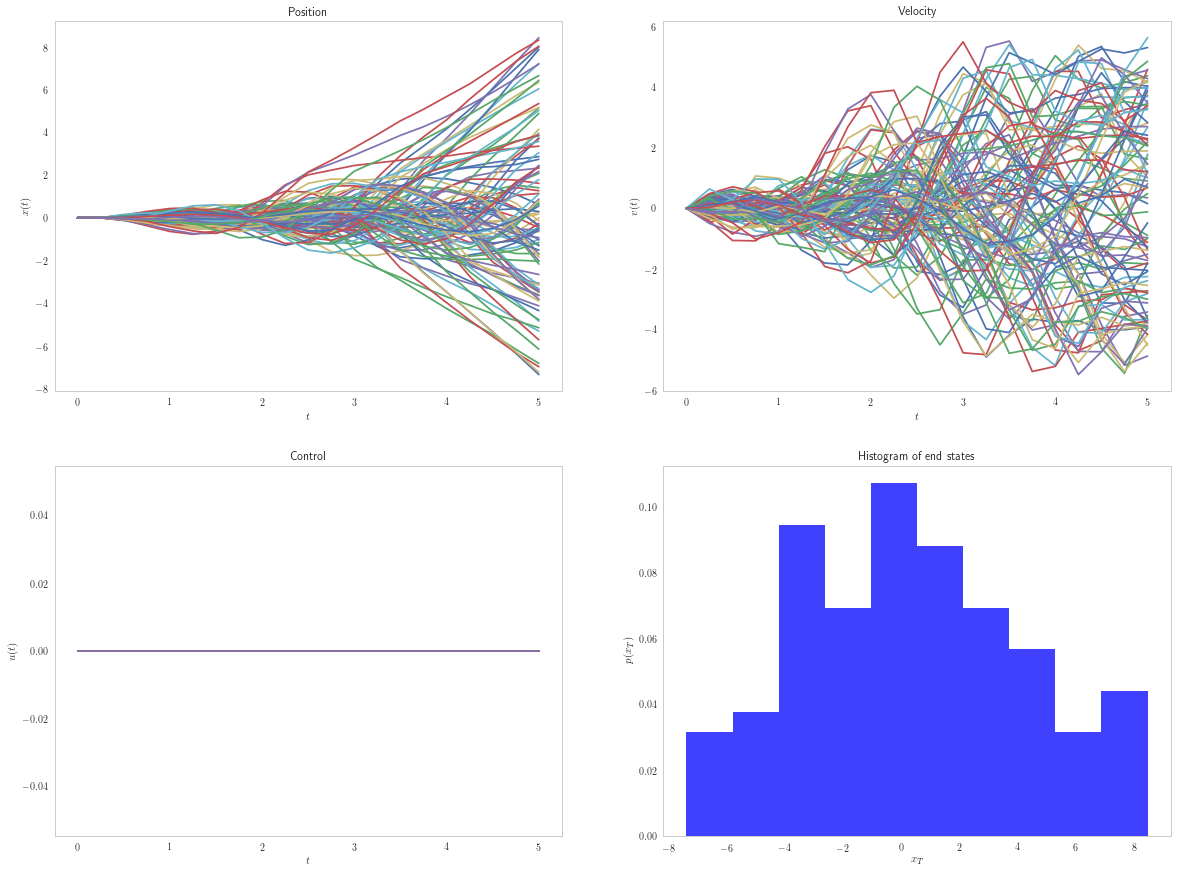
\includegraphics[width=300px]{f1.png}
\caption{$100$ simulations without control (so $u=0$) with $(x_0, v_0) = (0, 0)$, $A=-1$, $R=1$, $\nu=0.2$, $T=5$, $g=-10$ and $dt=0.25$.}
\label{fig:mcp-f1}
\end{figure}

\begin{figure}[h]
\centering
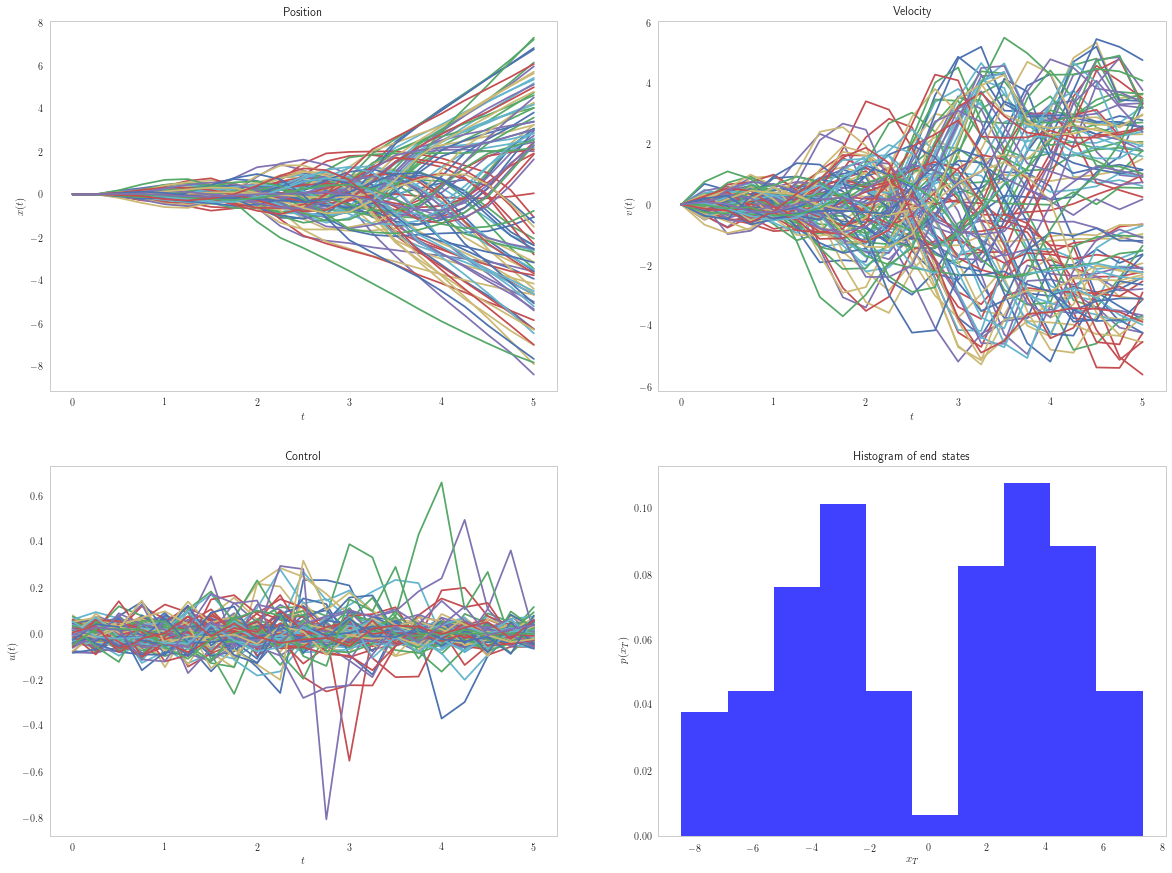
\includegraphics[width=300px]{f2.png}
\caption{$100$ simulations with optimal control (computed with $100$ samples per timestep) with $(x_0, v_0) = (0, 0)$, $A=-1$, $R=1$, $\nu=0.2$, $T=5$, $g=-10$ and $dt=0.25$.}
\label{fig:mcp-f2}
\end{figure}

In figure \ref{fig:mcp-f1} and \ref{fig:mcp-f2}, there clearly is a difference in the end states for simulations without any control (so $u=0$) and in simulations with optimal control. Optimal control resulted in only a few simulations in which $-2 < x_T < 2$. Most of the simulations escaped the valley. It is also interesting to see that the control is kept fairly small. The heaviest controls are performed after some time. Here, the delayed choice mechanism also applies because of that.

\section{Discussions and conclusions}
For both problems, the delayed choice mechanism applies. It is not optimal for the control, to steer the system into a direction, since noise can cancel these effects. If the noise is too large, the no control is applied at all.

For the controlled random walk problem, it was easy to gain insights into the dynamics of the system by looking at the formula. The results were verified by running many simulations. For extremely large noise ($v \rightarrow \infty$), the optimal control goes to zero. The more $t \rightarrow T$, the more control is performed. The delayed control mechanism is caused by the fact that control has more influence at the end state at a relatively late point in time than control which is performed at the beginning of the time.

The second-order differential equations in the mountain car problem made the problem quite hard analytically. However, by approximating the optimal control by using MCMC sampling, we obtained satisfying results.

\newpage
\section{Appendix}
\subsection{Code for the controlled random walk (MATLAB)}
\lstinputlisting{../Control.m}

\subsection{Code for the mountain car problem (iPython Notebook)}
\subsubsection{Imports}
\begin{lstlisting}[language=Python]
import numpy as np
import math
import matplotlib.pyplot as plt
from matplotlib import rc
import seaborn as sns
import numpy as np
import matplotlib.pyplot as plt
from matplotlib import animation, rc
from IPython.display import HTML

% matplotlib inline

rc('text', usetex=True)
sns.set_style("whitegrid", {'axes.grid' : False})
\end{lstlisting}

\subsection{Definitions}
\begin{lstlisting}[language=Python]
def L(x):
    # The definition of the valley
    return -1 - 0.5 * (np.tanh(2 * x + 2) - np.tanh(2 * x - 2))
    
def sech(x):
    # The sech function
    return 2. / (np.exp(x) + np.exp(-x))

def dLdx(x):
    # dL / dx evaluated at point x
    return np.power(sech(2 * x + 2), 2) - np.power(sech(2 * x - 2), 2)
    
def F(x, g):
    # The gravitational force
    return -g * dLdx(x) / np.sqrt(1 + np.power(dLdx(x), 2))
\end{lstlisting}

\subsection{Base class for simulations}
\begin{lstlisting}[language=Python]
class MountainCarProblem:
    
    def __init__(self, x_0, v_0, A=-1, R=1, nu=1, T=1, g=1, dt=0.01, u=0, t_0=0):
        """
        Initialize the Mountain Car Problem.
        
        x_0: The initial position.
        v_0: The initial velocity.
        A:   The reward for ending outside the valley (default: -1).
        R:   Relation between the noise level and the optimal control (default: 1).
        nu:  Noise level.
        T:   Horizon.
        g:   Gravitational constant (default: 1).
        u:   Constant control (default: 0). For dynamic control, implement the compute_control method.
        t_0: The start time of the system such that 0 <= t_0 <= T (default: t_0=0).
        """
        self.x_0, self.v_0, self.A, self.R, self.nu, self.T, self.g, self.dt, self.u, self.t_0 = x_0, v_0, A, R, nu, T, g, dt, u, t_0
        self.x_min, self.x_max = -2, 2
        self.x = self.x_0
        self.v = self.v_0
        self.t = self.t_0
        
    def run(self):
        """
        Run the simulation. It will return the following result:
        
        [xs, vs, ts, dus, dxis] in which:
        xs:   The computed positions over time.
        vs:   The computed velocities over time.
        ts:   The computed times (simply ranging from 0 to T).
        dus:  The computed controls over time.
        dxis: The computed noise per timestep.
        """
        xs, vs, ts, dus, dxis = [], [], [], [], []
        x, v, t = self.x_0, self.v_0, self.t_0
        steps = math.floor((self.T - self.t_0) / self.dt) + 1
        
        for step in range(steps):
            dudt = self.compute_control()
            noise = 0 if self.nu == 0 else np.random.normal(0, self.nu)
            dxi = np.sqrt(self.dt) * noise
            
            xs.append(x)
            vs.append(v)
            ts.append(t)
            dus.append(dudt)
            dxis.append(dxi)
            
            dx = v * self.dt
            dv = F(x, self.g) * self.dt + dudt + dxi
            
            x += dx
            v += dv
            t += self.dt
            
            self.x = x
            self.v = v
            self.t = t
            
        phi = 0 if self.x_min < self.x and self.x < self.x_max else self.A
            
        return xs, vs, ts, dus, dxis, phi
        
    def compute_control(self):
        """
        Compute the control. This method has access to state variables self.x (position), self.v (velocity) and self.t (time).
        """
        return self.u
\end{lstlisting}

\subsection{Optimal Control}
\begin{lstlisting}
class OptimalControlMCP(MountainCarProblem):
    def run_uncontrolled(self, x, v, t):
        mcp = MountainCarProblem(x_0=x, v_0=v, A=self.A, R=self.R, nu=self.nu, T=self.T, g=self.g, dt=self.dt, u=0, t_0=t)
        return mcp.run()
    
    def compute_control(self):
        w = []
        xi = []
        N = 100
        for _ in range(N):
            xs, vs, ts, dus, dxis, phi = self.run_uncontrolled(self.x, self.v, self.t)
            step = math.floor(self.t / self.dt)
            if len(dxis) > 0:
                dxis = np.asarray(dxis)
                if phi == 0:
                    w.append(0)
                else:
                    w.append(1. / N * np.exp(-phi))
                xi.append(dxis[0])
            else:
                w.append(0)
        w = np.array(w)
        xi = np.array(xi)
        ones = np.ones(w.shape)
        denom = np.dot(w, ones)
        if denom == 0:
            return 0
        udt = np.dot(w, xi) / denom
        return udt
\end{lstlisting}

\subsection{Approximating $J(x, v, t=0)$}
\begin{lstlisting}
xs = np.linspace(-2, 2, 41)
vs = np.linspace(-2, 2, 41)
n = 100
Js = []

for x in xs:
    row = []
    for v in vs:
        S = 0
        for mu in range(n):
            mcp = MountainCarProblem(x, v, nu=4, g=-10, u=0, A=-1)
            _, _, ts, dus, dxis, phi = mcp.run()
            S += np.exp(-phi)
        S /= n
        J = -np.log(S)
        row.append(J)
    Js.append(row)

fig, ax = plt.subplots(1, 1)
plt.imshow(Js, cmap='hot', extent=(-2, 2, -2, 2))
plt.colorbar()
plt.xlabel('$x$')
plt.ylabel('$v$')
\end{lstlisting}
\end{document}